\documentclass[class=minimal,border=0pt]{standalone}\usepackage[utf8]{inputenc}
\usepackage{amsmath}
\usepackage{amsfonts}
\usepackage{amssymb}
\usepackage{tikz-qtree,tikz-qtree-compat}
\begin{document}

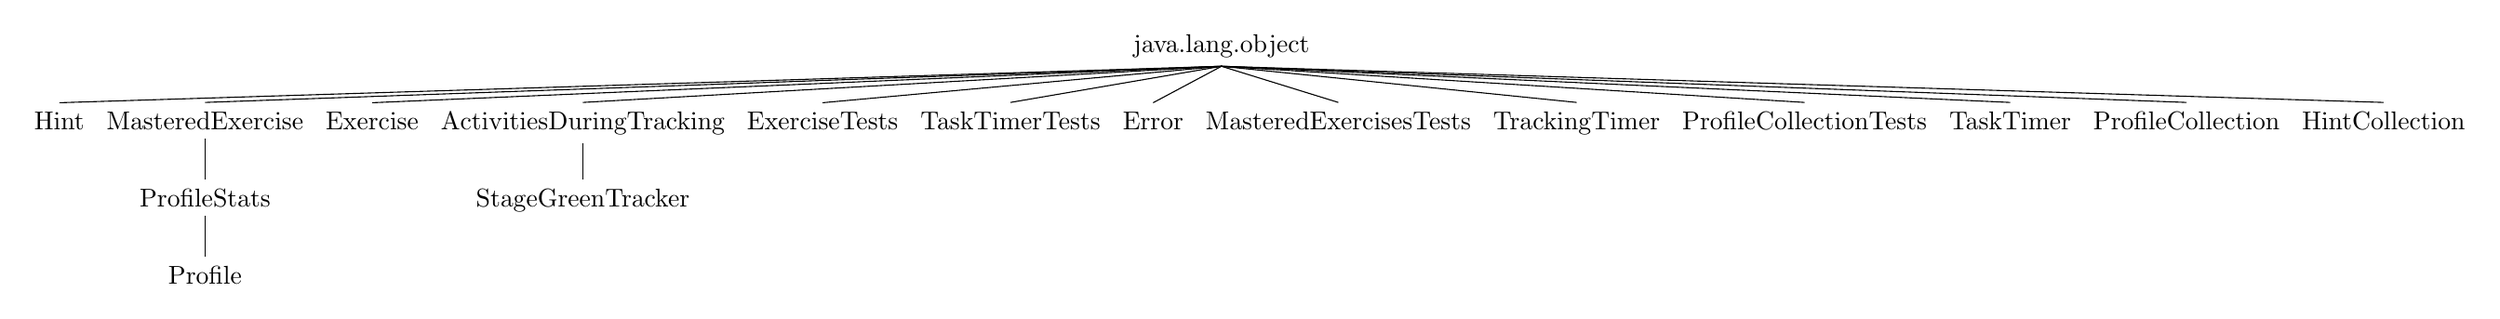
\begin{tikzpicture}
\Tree[.java.lang.object
		[.Hint
	]
		[.MasteredExercise
				[.ProfileStats
						[.Profile
			]
		]
	]
		[.Exercise
	]
		[.ActivitiesDuringTracking
				[.StageGreenTracker
		]
	]
		[.ExerciseTests
	]
		[.TaskTimerTests
	]
		[.Error
	]
		[.MasteredExercisesTests
	]
		[.TrackingTimer
	]
		[.ProfileCollectionTests
	]
		[.TaskTimer
	]
		[.ProfileCollection
	]
		[.HintCollection
	]
]
\end{tikzpicture}
%Stage
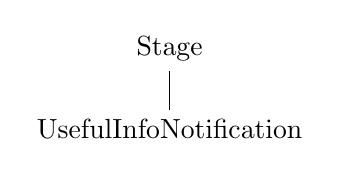
\begin{tikzpicture}
\Tree[.Stage
		[.UsefulInfoNotification
	]
]
\end{tikzpicture}
%Application
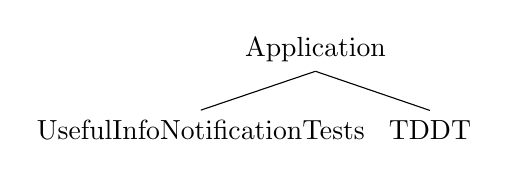
\begin{tikzpicture}
\Tree[.Application
		[.UsefulInfoNotificationTests
	]
		[.TDDT
	]
]
\end{tikzpicture}
%EventHandler<ActionEvent>
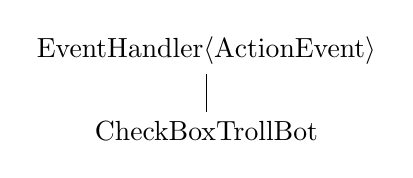
\begin{tikzpicture}
\Tree[.EventHandler$\langle$ActionEvent$\rangle$
		[.CheckBoxTrollBot
	]
]
\end{tikzpicture}
%TimerTask
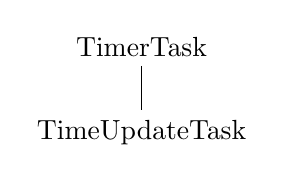
\begin{tikzpicture}
\Tree[.TimerTask
		[.TimeUpdateTask
	]
]
\end{tikzpicture}

\end{document}%This .tex file was written with Heretikz!
%Remember to include 
%java.lang.object
